%%%%%%%%%%%%%%%%%%%%%%%%%%%%%%%%%%%%%%%%%%%%%%%%%%%%%%%%%%%%%%%%%%%%%%%%%%%%%%%%%%%%%%%%%%%%%%%%%%%%
  \section{Introducci\'on}
  \begin{frame}
    \frametitle{Introducci\'on}
    FTP proviene de las siglas en inglés de File Transfer Protocol. Es un protocolo utilizado en forma específica para la transferencia de archivos a través de una red. \\
  \end{frame}

  \begin{frame}
    \frametitle{FTP y sus variantes}
    \begin{columns}[t]
     \column{0.4\textwidth}
     {\bf FTPS}. Es una de las variantes del protocolo FTP utilizadas para la transmisión de datos de forma segura y cifrada por la red. En este protocolo, cada camino implica el uso de una capa SSL / TLS por debajo del protocolo FTP estándar para cifrar la información de control del servidor y/o los canales de datos.
     
     \column{0.4\textwidth}
     {\bf SFTP}. Es otra variante del protocolo FTP para la transmisión de datos segura. Se utiliza habitualmente con el protocolo SSH para proporcionar dicha transferencia segura de archivos, aunque también puede utilizarse con otros protocolos de transferencia de datos seguros.
     \end{columns}
  \end{frame}


  \begin{frame}
    \frametitle{vsFTPd}
    Very secure File Transfer Protocol daemon, es probablemente el servidor FTP m\'as seguro y r\'apido para sistemas Unix, tiene una licencia GPL y cuenta con diferentes caracter\'isticas, algunas son las siguientes:
    \begin{itemize}
    \item Usuarios virtuales.
    \item Potente capacidad de configuracion por usuario.
    \item Limite de ancho de banda.
    \item Configuracion por IP de origen.
    \item Limite por IP de origen
    \item IPv6.
    \item Soporte de cifrado a través de la integración SSL({\em Secure Sockets Layer}).
  	\end{itemize}
  \end{frame}

%%%%%%%%%%%%%%%%%%%%%%%%%%%%%%%%%%%%%%%%%%%%%%%%%%%%%%%%%%%%%%%%%%%%%%%%%%%%%%%%%%%%%%%%%%%%%%%%%%%%
  \section{Sistema Operativo Utilizado}
  \begin{frame}
    \frametitle{Sistema Operativo Utilizado}
    El sistema operativo que se utilizó para montar y configurar el servidor vsftpd fue: Debian 8.
     \begin{figure}
      \centering
      
\includegraphics[width=0.3\textwidth]{./image/debian.png}
      \label{fig:ejemplo}
      \end{figure}
  \end{frame}
%%%%%%%%%%%%%%%%%%%%%%%%%%%%%%%%%%%%%%%%%%%%%%%%%%%%%%%%%%%%%%%%%%%%%%%%%%%%%%%%%%%%%%%%%%%%%%%%%%%%
  \section{Tecnolog\'ias$/$ Puertos $/$ Protocolos}
%\subsection{Tecnologias}
%  \begin{frame}
%    \frametitle{Tecnolog\'ias}
%    \begin{itemize}
%    	\item 
%    \end{itemize}
%  \end{frame}

\subsection{Puertos y Protocolos}
\begin{frame}
\normalsize
  	\frametitle{Puertos utilizados según los modos de conexión de FTP.}
  	\begin{itemize}
  	\item {\bf Activo}. El cliente crea una conexión de datos a través del puerto 20 del servidor, mientras que en el cliente asocia esta conexión desde un puerto aleatorio entre 1024 y 65535, enviando PORT para indicar al servidor el puerto a utilizar para la transferencia de datos.

  	\item {\bf Pasivo}. El cliente envía PASV en lugar de PORT a través del puerto de control del servidor(21). Éste devuelve como respuesta el número de puerto a través del cual debe conectarse el cliente para hacer la transferencia de datos. El servidor puede elegir al azar cualquier puerto entre 1024 y 65535 o bien el rango de puertos determinado por el administrador del sistema.
  	\end{itemize}
\end{frame}

%%%%%%%%%%%%%%%%%%%%%%%%%%%%%%%%%%%%%%%%%%%%%%%%%%%%%%%%%%%%%%%%%%%%%%%%%%%%%%%%%%%%%%%%%%%%%%%%%%%%
  %%%%%%%%%%%%%%%%%%%%%%%%%%%%%%%%%%%%%%%%%%%%%%%%%%%%%%%%%%%%%%%%%%%%%%%%%%%%%%%%%%%%%%%%%%%%%%%%%%%%
\section{Instalaci\'on}
  \begin{frame}
    \frametitle{Instalaci\'on}
    

    
  \end{frame}
%%%%%%%%%%%%%%%%%%%%%%%%%%%%%%%%%%%%%%%%%%%%%%%%%%%%%%%%%%%%%%%%%%%%%%%%%%%%%%%%%%%%%%%%%%%%%%%%%%%%

  \section{Instalaci\'on de vsftpd}
  \begin{frame}
    \frametitle{Instalaci\'on}
		
  \end{frame}
%%%%%%%%%%%%%%%%%%%%%%%%%%%%%%%%%%%%%%%%%%%%%%%%%%%%%%%%%%%%%%%%%%%%%%%%%%%%%%%%%%%%%%%%%%%%%%%%%%%%
  %%%%%%%%%%%%%%%%%%%%%%%%%%%%%%%%%%%%%%%%%%%%%%%%%%%%%%%%%%%%%%%%%%%%%%%%%%%%%%%%%%%%%%%%%%%%%%%%%%%%
\section{Configuraci\'on}

  \begin{frame}
    \frametitle{Configuraci\'on}
    \begin{itemize}
      \item Respaldo del archivo de vsftpd.conf
      \item Se crea un shell virtual o fantasma.
      \item Se agrega un grupo que controle al servicio de vsftpd.
    \end{itemize}
    \begin{shell}
      \cmd{ cp /etc/vsftpd.conf /etc/vsftpd.conf.backup }\\
      \cmd{ mkdir /bin/ftp }
      \cmd{ sh -c \tqd echo ''/bin/ftp'' >> /etc/shells\tqd}\\
      \cmd{ groupadd ftp }
      \cmd{ mkdir /home/ftp }
    \hline\end{shell}
  \end{frame}
%%%%%%%%%%%%%%%%%%%%%%%%%%%%%%%%%%%%%%%%%%%%%%%%%%%%%%%%%%%%%%%%%%%%%%%%%%%%%%%%%%%%%%%%%%%%%%%%%%%%

  \begin{frame}
    \frametitle{Configuraci\'on}
    \begin{itemize}
      \item Crear el home donde cada usuario va encontrar su informaci\'on.
      \item Se crea un directorio en el home de cada usuario, al cual se le dar\'an permisos, para 
      que pueda subir archivos o crear directorios mediante ftp.
      \item Se modifica los permisos a las carpetas y la propiedad de las mismas.
    \end{itemize}
    
    \begin{shell}
      \cmd{ mkdir /home/ftp/usuario }
      \cmd{ chmod 555 /home/ftp/usuario }\\
      \cmd{ mkdir /home/ftp/usuario/upload }
      \cmd{ chmod 0755 /home/ftp/usuario/upload }
    \hline\end{shell}
  \end{frame}
%%%%%%%%%%%%%%%%%%%%%%%%%%%%%%%%%%%%%%%%%%%%%%%%%%%%%%%%%%%%%%%%%%%%%%%%%%%%%%%%%%%%%%%%%%%%%%%%%%%%

   \begin{frame}
     \frametitle{Configuraci\'on}
    \begin{itemize}
      \item Se crea el nuevo usuario.
      \begin{itemize}
        \item Se agrega al grupo ftp.
        \item Se le asigna su directorio home.
        \item Se le asigna el shell virtual.
      \end{itemize}
      \item Se modifica la propiedad de las carpetas del home.
    \end{itemize}
    
    \begin{shell}
      \cmd{ useradd -g ftp -d /home/ftp/usuario -s /bin/ftp -c ''Nombre del usuario'' usuario }\\
      \cmd{ chown usuario.ftp /home/ftp/usuario/* -R }
    \hline\end{shell}
   \end{frame}
%%%%%%%%%%%%%%%%%%%%%%%%%%%%%%%%%%%%%%%%%%%%%%%%%%%%%%%%%%%%%%%%%%%%%%%%%%%%%%%%%%%%%%%%%%%%%%%%%%%%

   \begin{frame}
     \frametitle{Configuraci\'on}
     \framesubtitle{Archivo vsftpd.chroot\_list}
     \begin{itemize}
       \item Crear el archivo vsftpd.chroot\_list
       \item Agregar el usuario al archivo, tal como esta en /etc/passwd
     \end{itemize}
    \begin{shell}
      \cmd{ touch /etc/vsftpd.chroot\_list }
      \cmd{ sh -c \tqd cat /etc/passwd | grep usuario >> /etc/vsftpd.chroot\_list \tqd }
    \hline\end{shell}
   \end{frame}
%%%%%%%%%%%%%%%%%%%%%%%%%%%%%%%%%%%%%%%%%%%%%%%%%%%%%%%%%%%%%%%%%%%%%%%%%%%%%%%%%%%%%%%%%%%%%%%%%%%%

  \begin{frame}
    \frametitle{Configuraci\'on}
    \framesubtitle{Archivo vsftpd.conf}
    Se modifica algunas opciones en el archivo de configuraci\'on.
    \begin{shell}\\
      listen=YES\\
      local\_enable=YES\\
      write\_enable=YES\\
      xferlog\_file=/var/log/vsftpd.log\\
      ftpd\_banner=Welcome to Equipo-7 FTP service.\\ \\
    \hline\end{shell}
   \end{frame}
   
%%%%%%%%%%%%%%%%%%%%%%%%%%%%%%%%%%%%%%%%%%%%%%%%%%%%%%%%%%%%%%%%%%%%%%%%%%%%%%%%%%%%%%%%%%%%%%%%%%%%

    \begin{frame}
    \frametitle{Configuraci\'on}
    \framesubtitle{Archivo vsftpd.conf}
    Con estas configuraciones limitamos a cada usuario a su directorio personal.
    \begin{shell}\\
      chroot\_local\_user=YES\\
      chroot\_list\_enable=YES\\
      chroot\_list\_file=/etc/vsftpd.chroot\_list\\ \\
    \hline\end{shell}
   \end{frame}
   
%%%%%%%%%%%%%%%%%%%%%%%%%%%%%%%%%%%%%%%%%%%%%%%%%%%%%%%%%%%%%%%%%%%%%%%%%%%%%%%%%%%%%%%%%%%%%%%%%%%%

  \begin{frame}
    \frametitle{Configuraci\'on}
    \framesubtitle{FTPS}
    Se crea las llaves.
    
    \begin{shell}
      \cmd{openssl req -sha256 -x509 -nodes -days 365 -newkey rsa:4096 
      -keyout /etc/ssl/private/vsftpd.key -out /etc/ssl/certs/vsftpd.pem}\\
    \hline\end{shell}
    
    Se modifica algunas opciones en el archivo de configuraci\'on.
    
    \begin{shell}
      rsa\_cert\_file=/etc/ssl/certs/vsftpd.pem\\
      rsa\_private\_key\_file=/etc/ssl/private/vsftpd.key\\
      ssl\_enable=YES\\
    \hline\end{shell}
   \end{frame}
   
%%%%%%%%%%%%%%%%%%%%%%%%%%%%%%%%%%%%%%%%%%%%%%%%%%%%%%%%%%%%%%%%%%%%%%%%%%%%%%%%%%%%%%%%%%%%%%%%%%%%

%%%%%%%%%%%%%%%%%%%%%%%%%%%%%%%%%%%%%%%%%%%%%%%%%%%%%%%%%%%%%%%%%%%%%%%%%%%%%%%%%%%%%%%%%%%%%%%%%%%%
  \section{Instalacion de cliente}
  \begin{frame}
    \frametitle{Clientes}
    \begin{itemize}
    	\item Cientes con entorno gr\'afico.
		\begin{itemize}
	   	 \item Filezilla. Para Linux, Windows y MacOS.\\
	   	 	Desde bash de Debian:
	   	 	\begin{shell}
	     	  \cmd{ apt-get update }
	     	 \\ \cmd{ apt-get -y install filezilla }\\
	    	\hline\end{shell}
	   	 \item WinSCP. Solo windows.
	    \end{itemize}

	    \item Clientes para android.
		\begin{itemize}
	   	 \item ES File Explorer.
	   	 \item AndFTP.
	   	 \item TurboFTP. 
	    \end{itemize}
	   	\item Comando {\bf ftp} en bash linux y ms-dos de windows.
	  \end{itemize}
  \end{frame}
%%%%%%%%%%%%%%%%%%%%%%%%%%%%%%%%%%%%%%%%%%%%%%%%%%%%%%%%%%%%%%%%%%%%%%%%%%%%%%%%%%%%%%%%%%%%%%%%%%%%
  %%%%%%%%%%%%%%%%%%%%%%%%%%%%%%%%%%%%%%%%%%%%%%%%%%%%%%%%%%%%%%%%%%%%%%%%%%%%%%%%%%%%%%%%%%%%%%%%%%%%%%%%%%%%%%%%%%%%%%%%
\section{Diagrama}
  \begin{frame}
    \frametitle{Diagrama}
      \begin{figure}
      \centering
      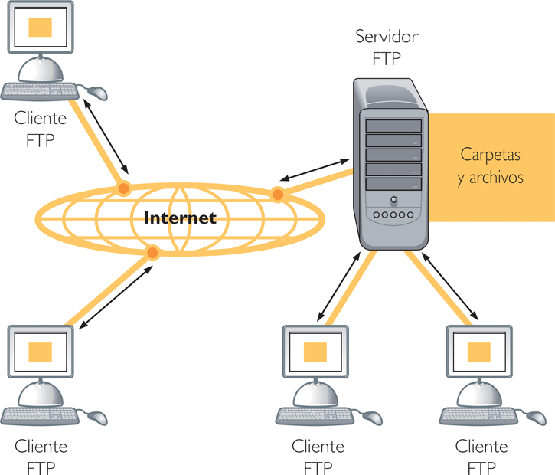
\includegraphics[width=0.5\textwidth]{./image/diagramaFTP.png}
      \label{fig:ejemplo}
      \end{figure}
  \end{frame}
%%%%%%%%%%%%%%%%%%%%%%%%%%%%%%%%%%%%%%%%%%%%%%%%%%%%%%%%%%%%%%%%%%%%%%%%%%%%%%%%%%%%%%%%%%%%%%%%%%%%
  \section{Configuraci\'on de red}
  \begin{frame}
    \frametitle{Configuraci\'on de red}
      \begin{figure}
      \centering
      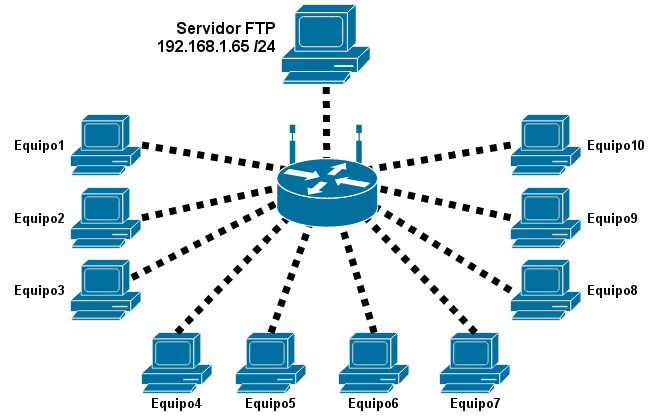
\includegraphics[width=0.8\textwidth]{./image/configuracionRed.png}
      \label{fig:ejemplo1}
      \end{figure}
  \end{frame}
%%%%%%%%%%%%%%%%%%%%%%%%%%%%%%%%%%%%%%%%%%%%%%%%%%%%%%%%%%%%%%%%%%%%%%%%%%%%%%%%%%%%%%%%%%%%%%%%%%%%
\section{Servidor}
  \begin{frame}
    \frametitle{Servidor}
    algo
  \end{frame}
%%%%%%%%%%%%%%%%%%%%%%%%%%%%%%%%%%%%%%%%%%%%%%%%%%%%%%%%%%%%%%%%%%%%%%%%%%%%%%%%%%%%%%%%%%%%%%%%%%%%
%\section{Tecnolog\'ias de comunicaci\'on}
%  \begin{frame}
%    \frametitle{Tecnolog\'ias de comunicaci\'on}
%  \end{frame}
%%%%%%%%%%%%%%%%%%%%%%%%%%%%%%%%%%%%%%%%%%%%%%%%%%%%%%%%%%%%%%%%%%%%%%%%%%%%%%%%%%%%%%%%%%%%%%%%%%%%
\section{Equipos utilizados}
  \begin{frame}
    \frametitle{Equipos utilizados}
    \begin{itemize}
      \item Servidor HP-Ultrabook Modelo: 
      \item Switch: 
    \end{itemize}
  \end{frame}
%%%%%%%%%%%%%%%%%%%%%%%%%%%%%%%%%%%%%%%%%%%%%%%%%%%%%%%%%%%%%%%%%%%%%%%%%%%%%%%%%%%%%%%%%%%%%%%%%%%%
\section{Demostración}
\begin{frame}
  \frametitle{¿Qué hora es?}
  \centering
  \large !Hora de la demostración!
\end{frame}

%%%%%%%%%%%%%%%%%%%%%%%%%%%%%%%%%%%%%%%%%%%%%%%%%%%%%%%%%%%%%%%%%%%%%%%%%%%%%%%%%%%%%%%%%%%%%%%%%%%%
%\section{Pruebas de funcionamiento}
%  \begin{frame}
%    \frametitle{Pruebas de funcionamiento}
%    algo
%  \end{frame}
%%%%%%%%%%%%%%%%%%%%%%%%%%%%%%%%%%%%%%%%%%%%%%%%%%%%%%%%%%%%%%%%%%%%%%%%%%%%%%%%%%%%%%%%%%%%%%%%%%%%%%%%%%%%%%%%%%%%%%%%
%\section{Pruebas de Comunicaci\'on}
%  \begin{frame}
%    \frametitle{Pruebas de Comunicaci\'on}
%    algo
%  \end{frame}
%%%%%%%%%%%%%%%%%%%%%%%%%%%%%%%%%%%%%%%%%%%%%%%%%%%%%%%%%%%%%%%%%%%%%%%%%%%%%%%%%%%%%%%%%%%%%%%%%%%%%%%%%%%%%%%%%%%%%%%%
%\section{Pruebas de funcionamiento de protocolos}
%  \begin{frame}
%    \frametitle{Pruebas de funcionamiento de protocolos}
%    algo
%  \end{frame}
%%%%%%%%%%%%%%%%%%%%%%%%%%%%%%%%%%%%%%%%%%%%%%%%%%%%%%%%%%%%%%%%%%%%%%%%%%%%%%%%%%%%%%%%%%%%%%%%%%%%%%%%%%%%%%%%%%%%%%%%
%\section{Analizador de protocolos}
%  \begin{frame}
%    \frametitle{Analizador de protocolos}
%    algo
%  \end{frame}
%%%%%%%%%%%%%%%%%%%%%%%%%%%%%%%%%%%%%%%%%%%%%%%%%%%%%%%%%%%%%%%%%%%%%%%%%%%%%%%%%%%%%%%%%%%%%%%%%%%%%%%%%%%%%%%%%%%%%%%%
%\section{Estad\'isticas}
%  \begin{frame}
%    \frametitle{Estad\'isticas}
%    algo
%  \end{frame}
%%%%%%%%%%%%%%%%%%%%%%%%%%%%%%%%%%%%%%%%%%%%%%%%%%%%%%%%%%%%%%%%%%%%%%%%%%%%%%%%%%%%%%%%%%%%%%%%%%%%%%%%%%%%%%%%%%%%%%%%
%\section{Errores}
%  \begin{frame}
%    \frametitle{Errores}
%    algo
%  \end{frame}
%%%%%%%%%%%%%%%%%%%%%%%%%%%%%%%%%%%%%%%%%%%%%%%%%%%%%%%%%%%%%%%%%%%%%%%%%%%%%%%%%%%%%%%%%%%%%%%%%%%%%%%%%%%%%%%%%%%%%%%%
\section{Capacidad del canal y velocidad de comunicaci\'on}
  \begin{frame}
    \frametitle{Capacidad del canal y velocidad de comunicaci\'on}       
      Normas: IEEE 802.11n*,IEEE 802.11g,IEEE 802.11b\\
      Tasas de señal inalámbrica: Hasta 150Mbps\\
      Rango de frecuencia: 2.4-2.4835GHz\\
      Potencia de transmisión inalámbrica:20dBm(max. EIRP)**\\
      Tecnología de modulación: DBPSK,DQPSK,CCK,OFDM,\\
      16-QAM,64-QAM\\
  \end{frame}
%%%%%%%%%%%%%%%%%%%%%%%%%%%%%%%%%%%%%%%%%%%%%%%%%%%%%%%%%%%%%%%%%%%%%%%%%%%%%%%%%%%%%%%%%%%%%%%%%%%%%%%%%%%%%%%%%%%%%%%%
%\section{Trafico de Red}
%  \begin{frame}
%    \frametitle{Trafico de Red}
%    algo
%  \end{frame}
%%%%%%%%%%%%%%%%%%%%%%%%%%%%%%%%%%%%%%%%%%%%%%%%%%%%%%%%%%%%%%%%%%%%%%%%%%%%%%%%%%%%%%%%%%%%%%%%%%%%%%%%%%%%%%%%%%%%%%%%
\section{Conclusiones}
  \begin{frame}
    \frametitle{Conclusiones}
    El servidor ftp es de gran utilidad para compartir carpetas y archivos alojados quizás es un equipo remoto, y poder
    tenerlos disponibles en la red, siempre y cuando el servidor ftp esté en funcionamiento.
    La configuracion del servidor puede ser tan robusta como se pueda, va desde la configuracion del puerto por donde 
    el servidor estará a la escucha de peticiones, manejo de usuario y hasta enjaular usuarios, es decir, que no puedan 
    accesar a directorios ni archivos propios del servidor.

  \end{frame}
